\chapter{Experiments}
We now delve into out contribution to tackling the problem of automatic differential diagnosis of Mendelian diseases. At this scope we have prepared a tailored KG integrated with patient data, that we describe in \Cref{sec:patientKG}. We then outline how we have translated our problem into a link prediction task, motivating the choice of hyperbolic graph representation learning techniques (\Cref{sec:linkPredictionDiffDiagnosis}). 

\section{Patient KG}\label{sec:patientKG}
In this section we describe the data that we have chosen for the task of differential diagnosis of Mendelian diseases. We proceed by exploring the underlying biomedical knowledge graph that we have used and the patient data that we have selected. We also describe how these data sources have been integrated into a single knowledge graph.

\subsection{Underlying biomedical KG}
Initially we have considered PrimeKG \cite{chandak2023PrimeKG}, a knowledge graph targeted at precision medicine analyses aggregating 20 high quality resources. Unfortunately, at the moment of use we have encountered substantial shortcomings in the representation of Mendelian diseases. Taking inspiration from the entities represented in PrimeKG, we have constructed a tailored knowledge graph. We have resorted to \emph{PheKnowLator} (\emph{Phenotype Knowledge Translator})~\cite{callahan2020PheKnowlator}\footnote{The Python library is available at \url{https://github.com/callahantiff/PheKnowLator}}, a KG framework designed for optimized construction of semantically-rich, large-scale biomedical KGs accounting for different standardized terminologies or vocabularies. To construct our heterogenous graph we have selected various ontologies taking into account our final goal and memory constraints. The chosen ontologies, grouped by resulting node types, are the following.


\begin{multicols}{2}

\paragraph{Gene Ontology}
\begin{itemize}
\item Gene Ontology Chemical Entities (GOCHE)
\item Gene Ontology (GO)
\end{itemize}

\paragraph{Genomic Features}
\begin{itemize}
\item Ontology of Genes and Genomes (OGG)
\item Sequence Ontology (SO)
\end{itemize}

\paragraph{Proteins}
\begin{itemize}
\item Protein Ontology (PR)
\item Cell Ontology (CL)
\item Human Phenotype Ontology (HP)
\item Molecular Function (MF)
\end{itemize}
\bigskip

\paragraph{Diseases}
\begin{itemize}
\item Disease Ontology (DOID)
\item Mondo Disease Ontology (MONDO)
\end{itemize}
\bigskip

\paragraph{Phenotypes}
\begin{itemize}
\item Human Phenotype Ontology (HP)
\item Phenotype And Trait Ontology (PATO)
\item uPheno Ontology (UPHENO)
\end{itemize}
\end{multicols}
\begin{table}
    \centering
    \begin{tabular}{rr}
        \toprule
        \textbf{Node Type} & \textbf{\#} \\
        \midrule
        Protein & 122,740 \\
        GO & 40,803 \\
        Disease & 26,899 \\
        Genomic feature & 24,031 \\
        Phenotype & 19,645 \\
        \bottomrule
    \end{tabular}
    \caption{Distribution of node types in the knowledge graph}
    
    \label{tab:nodetypes}
\end{table}
\begin{table}
    \centering
    \begin{tabular}{lllr}
        \toprule
        \textbf{Edge Predicate} & \textbf{Subject} & \textbf{Object} & \textbf{\#} \\      
        \midrule
        Molecularly interacts with & Protein & Protein & 618,856 \\
        Phenotype of & Disease & Phenotype & 453,260 \\
        Has phenotype & Phenotype & Disease & 453,260 \\
        Subclassof & Protein & Protein & 164,224 \\
        Has participant & Protein & GO & 125,233 \\
        Participates in & GO & Protein & 125,230 \\
        Located in & GO & Protein & 81,468 \\
        Subclassof & GO & GO & 81,608 \\
        Location of & Protein & GO & 81,466 \\
        Has function & GO & Protein & 68,742 \\
        Function of & Protein & GO & 68,742 \\
        Subclassof & Disease & Disease & 45,251 \\
        Subclassof & Genomic feature & Genomic feature & 28,130 \\
        Subclassof & Phenotype & Phenotype & 25,852 \\
        Causes/contributes to condition & Phenotype & Genomic feature & 24,519 \\
        Has gene template & Genomic feature & Protein & 20,089 \\
        Gene product of & Genomic feature & Protein & 19,607 \\
        Has gene product & Protein & Genomic feature & 19,607 \\
        Causes/contributes to condition & Disease & Genomic feature & 14,418 \\
        Part of & GO & GO & 6,772 \\
        \bottomrule
    \end{tabular} 
    \caption{Distribution of (frequent) edge predicates per node type in the knowledge graph}   
    \label{tab:edgedistrib}
\end{table}
\begin{figure}
    \centering
    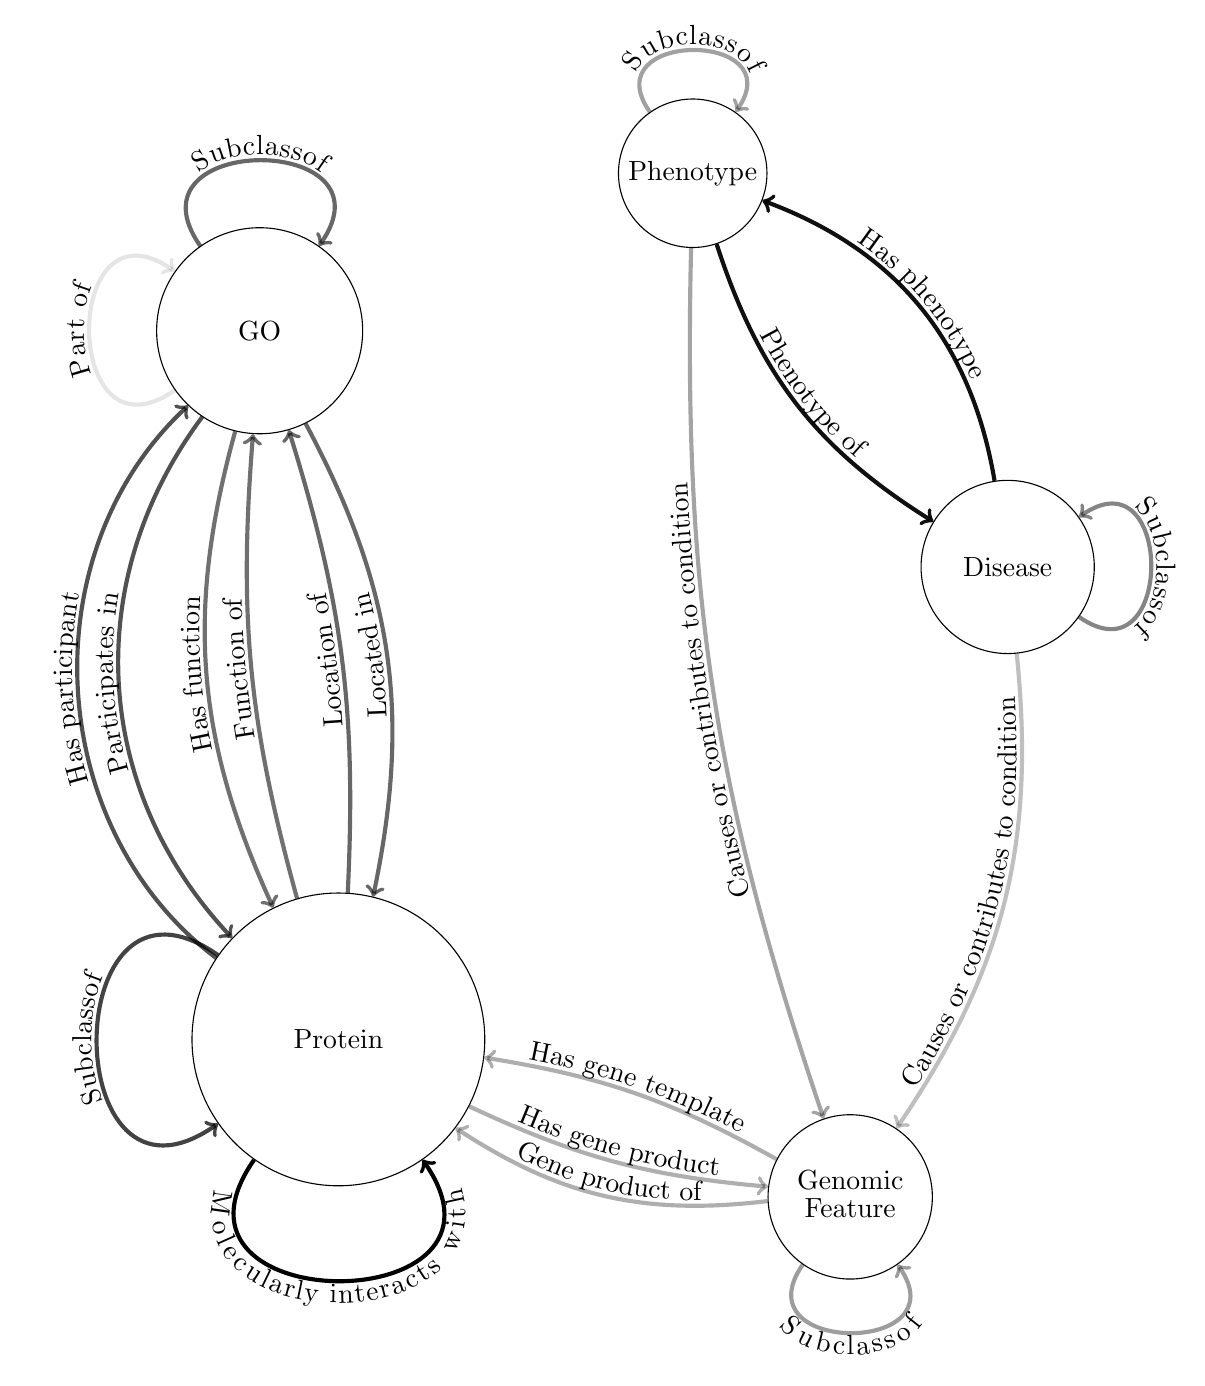
\begin{tikzpicture}
    \usetikzlibrary{decorations.text}

    \begin{scope}[xshift=1cm]
        % Nodes
        \node[circle, draw, fill=none, minimum size=3.718cm, inner sep=0pt] (Protein) at (-4,-3) {Protein};
        \node[circle, draw, fill=none, minimum size=2.617cm, inner sep=0pt] (GO) at (-5,6) {GO};
        \node[circle, draw, fill=none, minimum size=2.200cm, inner sep=0pt] (Disease) at (4.5,3) {Disease};
        \node[circle, draw, fill=none, minimum size=2.087cm, inner sep=0pt] (GenomicFeature) at (2.5,-5) {\begin{tabular}{c}Genomic\\[-0.5ex]Feature\end{tabular}};
        \node[circle, draw, fill=none, minimum size=1.886cm, inner sep=0pt] (Phenotype) at (0.5,8) {Phenotype};

        % Edges with curved labels
            \draw[->, line width=1.5pt, opacity=0.937927] (Disease) to[bend right=30] (Phenotype);
            \path[decorate, decoration={text along path, text align=center, raise=2pt, text={Has phenotype}}] (Phenotype) to[bend left=30] (Disease);

            \draw[->, line width=1.5pt, opacity=1.000000] (Protein) to[out=235, in=305, looseness=3] (Protein);
            \path[decorate, decoration={text along path, text align=center, raise=-8pt, text={Molecularly interacts with}}] (Protein) to[out=235, in=305, looseness=3](Protein);

            \draw[->, line width=1.5pt, opacity=0.478617] (Disease) to[out=-35, in=35, looseness=3] (Disease);
            \path[decorate, decoration={text along path, text align=center, raise=2pt, text={Subclassof}}] (Disease) to[out=35, in=-35, looseness=3] (Disease);

            \draw[->, line width=1.5pt, opacity=0.596164] (GO) to[out=125, in=55, looseness=3] (GO);
            \path[decorate, decoration={text along path, text align=center, raise=2pt, text={Subclassof}}] (GO) to[out=125, in=55, looseness=3] (GO);

            \draw[->, line width=1.5pt, opacity=0.383857] (GenomicFeature) to[out=235, in=305, looseness=3] (GenomicFeature);
            \path[decorate, decoration={text along path, text align=center, raise=-8pt, text={Subclassof}}] (GenomicFeature) to[out=235, in=305, looseness=3] (GenomicFeature);

            \draw[->, line width=1.5pt, opacity=0.367024] (Phenotype) to[out=125, in=55, looseness=3] (Phenotype);
            \path[decorate, decoration={text along path, text align=center, raise=2pt, text={Subclassof}}] (Phenotype) to[out=125, in=55, looseness=3] (Phenotype);

            \draw[->, line width=1.5pt, opacity=0.735558] (Protein) to[out=145, in=215, looseness=3] (Protein);
            \path[decorate, decoration={text along path, text align=center, raise=2pt, text={Subclassof}}] (Protein) to[out=215, in=145, looseness=3] (Protein);

            \draw[->, line width=1.5pt, opacity=0.561965] (Protein) to[bend left=10] (GO);
            \path[decorate, decoration={text along path, text align=center, raise=2pt, text={Function of}}] (Protein) to[bend left=10] (GO);


            \draw[->, line width=1.5pt, opacity=0.937927] (Phenotype) to[bend right=20] (Disease);
            \path[decorate, decoration={text along path, text align=center, raise=2pt, text={Phenotype of}}] (Phenotype) to[bend right=20] (Disease);

            \draw[->, line width=1.5pt, opacity=0.316749] (GenomicFeature) to[bend right=10] (Protein);
            \path[decorate, decoration={text along path, text align=center, raise=2pt, text={Has gene template}}] (Protein) to[bend left=10] (GenomicFeature);

            \draw[->, line width=1.5pt, opacity=0.561965] (GO) to[bend right=20] (Protein);
            \path[decorate, decoration={text along path, text align=center, raise=2pt, text={Has function}}] (Protein) to[bend left=20] (GO);

            \draw[->, line width=1.5pt, opacity=0.681528] (Protein) to[bend left=50] (GO);
            \path[decorate, decoration={text along path, text align=center, raise=2pt, text={Has participant}}] (Protein) to[bend left=50] (GO);

            \draw[->, line width=1.5pt, opacity=0.311908] (Protein) to[bend right=10] (GenomicFeature);
            \path[decorate, decoration={text along path, text align=center, raise=2pt, text={Has gene product}}] (Protein) to[bend right=10] (GenomicFeature);

           

            \draw[->, line width=1.5pt, opacity=0.595817] (Protein) to[bend right=10] (GO);
            \path[decorate, decoration={text along path, text align=center, raise=2pt, text={Location of}}] (Protein) to[bend right=10] (GO);

            \draw[->, line width=1.5pt, opacity=0.595822] (GO) to[bend left=20] (Protein);
            \path[decorate, decoration={text along path, text align=center, raise=2pt, text={Located in}}] (Protein) to[bend right=20] (GO);

            \draw[->, line width=1.5pt, opacity=0.681523] (GO) to[bend right=40] (Protein);
            \path[decorate, decoration={text along path, text align=center, raise=2pt, text={Participates in}}] (Protein) to[bend left=40] (GO);

            \draw[->, line width=1.5pt, opacity=0.250632] (Disease) to[bend left=20] (GenomicFeature);
            \path[decorate, decoration={text along path, text align=center, raise=2pt, text={Causes or contributes to condition}}] (GenomicFeature) to[bend right=20] (Disease);

            \draw[->, line width=1.5pt, opacity=0.356471] (Phenotype) to[bend right=10] (GenomicFeature);
            \path[decorate, decoration={text along path, text align=center, raise=2pt, text={Causes or contributes to condition}}] (GenomicFeature) to[bend left=10] (Phenotype);

            \draw[->, line width=1.5pt, opacity=0.311908] (GenomicFeature) to[bend left=20] (Protein);
            \path[decorate, decoration={text along path, text align=center, raise=2pt, text={Gene product of}}] (Protein) to[bend right=20] (GenomicFeature);

            \draw[->, line width=1.5pt, opacity=0.100000] (GO) to[out=215, in=145, looseness=3] (GO);
            \path[decorate, decoration={text along path, text align=center, raise=2pt, text={Part of}}] (GO) to[out=215, in=145, looseness=3] (GO);   \end{scope}
    \end{tikzpicture}

    \caption{A hypergraph representation of the underlying knowledge graph, having hypernodes representing the possibile node types and hyperedges for the most frequent edge predicates. The hypernodes' size and the hyperedges' opacity are logarithmic in the amount of node types and edge predicates respectively.}
    \label{fig:kg_hypergraph}
\end{figure}
The relations between the entities and their predicates derive from the annotations listed in the ontologies. 

In order of magnitude the knowledge graph has a total of $2.34\cdot10^5$ heterogeneus nodes and $2.71\cdot10^7$ heteorogeneous edges. The graph has a total of 6 node types and 117 edge predicates. In \Cref{fig:kg_hypergraph} we show the hypergraph representation of the knowledge graph obtained by aggregating the ontological data sources. To simplify the representation we have specified the edge predicates having at least $10^5$ occurrences in the whole knowledge graph. We specify the number of nodes for each type in \Cref{tab:nodetypes}, and in \Cref{tab:edgedistrib}, where we show the distribution of (the most frequent) edge predicates between node types.

\begin{figure}
    \centering
        \begin{tikzpicture}
        [edge from parent fork down,
        sibling distance=40mm,
        every node/.style={anchor=west, align=center}]
        \small
        \node {disease } 
        [sibling distance=30mm]
        child {node {human disease}
            [sibling distance=35mm] 
            child {node {digestive system disorder}
                [sibling distance=32mm]
                child {node {intestinal disorder}
                    [sibling distance=37mm]
                    child {node {intestinal obstruction}
                        [sibling distance=15mm]
                        child {node {ileus}
                            [sibling distance=27mm]
                            child {node {meconium ileus}    
                                [sibling distance=65mm]                 
                                    child {node {\small \textbf{cystic fibrosis associated meconium ileus}}}                                        
                                    child {node {\dots}}                    }
                            child {node {\dots}}
                       }
                        child {node {\dots}}
                   }
                    child {node {\dots}}
               }
                child {node {\dots}}
           }
            child {node {\dots}}
       }
        child {node {perinatal disease}
            [sibling distance=0mm]
            child {node {\small \textbf{cystic fibrosis associated meconium ileus}}}
       }
        child {node {\dots}};
    \end{tikzpicture}
    \caption{A subtree composed of disease type nodes linked by \emph{subclassof} edges centered on the leaf disease \emph{cystic fibrosis associated meconium ileus} .}
    \label{fig:SubclassofTree}
\end{figure}
One can observe that the graph is connected thanks to some edge predicates being one the symmetric of the other, e.g. \emph{has phenotype} and \emph{phenotype of}. Also, for each of the node types there are edges of predicate \emph{subclassof} that describe hierarchical relations between the entities. In \Cref{fig:SubclassofTree} we show a subtree of one of these hierarchical components in the knowledge graph. For other examples we suggest exploring the tree representations provided by the EMBL-EBI Ontology Lookup Service\footnote{Visit the EMBL-EBI Ontology Lookup Service at the link \url{https://www.ebi.ac.uk/ols4/}.}. One can imagine the knowledge graph made up of ``vertical'' components, one for each of the node types, as the one in the example. These hierarchies are interconnected by ``horizontal'' links that are agnostic to the hierarchical level of the nodes they are incident to. This characteristic has hinted us to the use of approaches based on hyperbolic geometry, as we will explore in \Cref{sec:hypPatientKG}.

\subsection{Patient data}
We have selected the patient data from the Phenopacket Store put together by~\cite{Danis2025Phenopackets}, consultable at the dedicated repository~\cite{Robinson2024PhenopacketStore}. We have based our analyses on the latest release to date, dating back to 19 January 2025 (version 0.1.24)\footnote{The phenopackets can be downloaded at \url{https://github.com/monarch-initiative/phenopacket-store/releases/download/0.1.24/all_phenopackets.zip}}, containing 7799 cohorts. 

The cohorts that represent the individuals with Mendelian diseases follow the GA4GH Phenopacket Schema~\cite{jacobsen2022ga4ghPhenopacketSchema}\footnote{In depth documentation can be found at \url{https://phenopacket-schema.readthedocs.io/en/latest/}}. The Phenopacket Schema represents an open standard for sharing disease and phenotype information useful for rare and common disease research. A Phenopacket links detailed phenotype descriptions with disease, patient, and genetic information, enabling human disease and biological understanding. 

For the patients collected in the Phenopacket Store the available attributes are listed below.
\begin{itemize}
  \item patient code
  \item sex
  \item age at last encounter
  \item phenotypes, with optional specification of the year of onset
  \item diagnosed disease, with optional specification of the year of onset and genomic interpretations
  \item reference to the research article
\end{itemize}

We have chosen to focus on features that are present in all cohorts, or described with similar level of detail. Therefore, we have discarded the year of onset of single phenotypes, the onset of the disease. In addition to genomic interpretations being not always present, this aspect will be covered by links contained in the underlying knowledge graph described in the previous section. We have also removed the age of last encounter of the patient since it is often unrelated with the diagnosed disease.

\subsection{Data integration}
The patient data has been integrated with the underling knowledge graph by adding nodes of type \emph{Person} and of type \emph{Article}. In particular, the \emph{Person} nodes comprehend the actual patients, and two nodes representing respectively the male and the female sex. For standardization purposes the \emph{Male} and \emph{Female} nodes are identified respectively using the IRIs \texttt{$\langle$http://purl.obolibrary.org/obo/NCIT\_C16576$\rangle$} and \texttt{$\langle$http://purl.obolibrary.org/obo/NCIT\_C20197$\rangle$}. Each article is indicated with \\ \texttt{$\langle$https://pubmed.ncbi.nlm.nih.gov/{article\_id}$\rangle$}. The nodes referring to patients expand on the \emph{Article} identifiers by adding the patient code, resulting in a string like \\ \texttt{$\langle$https://pubmed.ncbi.nlm.nih.gov/{article\_id}?{patient\_code}$\rangle$}. 

We clarify how the Phenopacket's data has been integrated with the underlying knowledge graph in \Cref{fig:patient_kg_hypergraph}, by specifying how the additional nodes have been connected among them and with the existing \emph{Phenotype} and \emph{Disease} nodes. From here on we will refer to the integrated knowledge graph as \emph{Patient KG}.

\begin{figure}
    \centering
    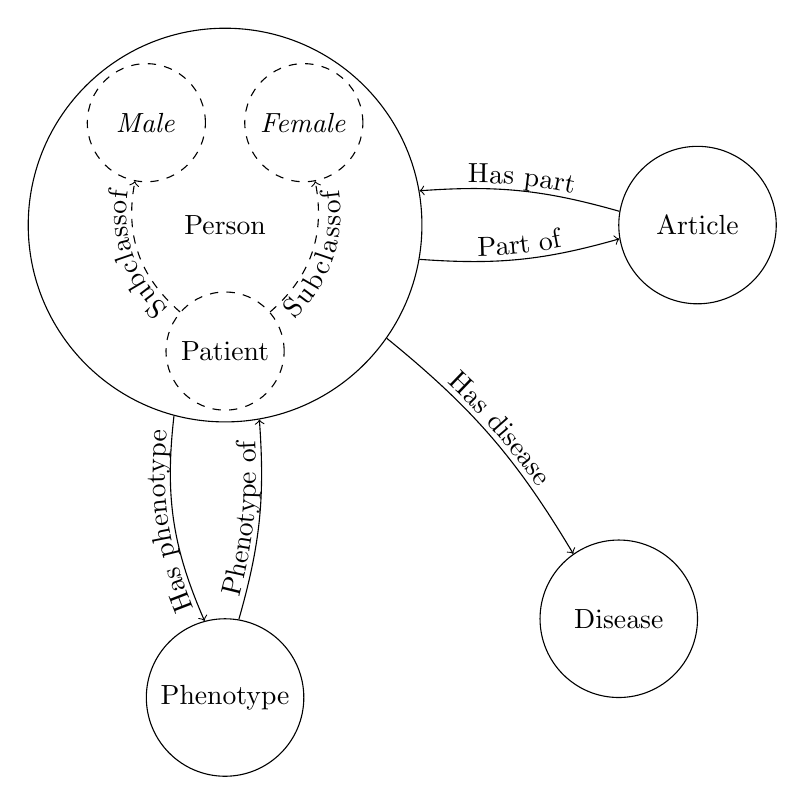
\begin{tikzpicture}
        % Nodes
        \node[circle, draw, fill=none, minimum size=2cm, inner sep=0pt] (Disease) at (1,4) {Disease};
        \node[circle, draw, fill=none, minimum size=2cm, inner sep=0pt] (Phenotype) at (-4,3) {Phenotype};
        \node[circle, draw, fill=none, minimum size=2cm, inner sep=0pt] (Article) at (2,9) {Article};
        \node[circle, draw, fill=none, minimum size=5cm, inner sep=0pt] (Person) at (-4,9) {Person};
        \node[circle, draw, dashed,  fill=none, minimum size=1.5cm, inner sep=0pt] (Male) at (-5,10.3) {\textit{Male}};
        \node[circle, draw, dashed, fill=none, minimum size=1.5cm, inner sep=0pt] (Female) at (-3,10.3) {\textit{Female}};
        \node[circle, draw, dashed, fill=none, minimum size=1.5cm, inner sep=0pt] (Patient) at (-4,7.4) {Patient};

        % Edges with curved labels
            \draw[->] (Person) to[bend right=10] (Article);
            \path[decorate, decoration={text along path, text align=center, raise=2pt, text={Part of}}] (Person) to[bend right=10] (Article);

            \draw[->] (Article) to[bend right=10] (Person);
            \path[decorate, decoration={text along path, text align=center, raise=2pt, text={Has part}}] (Person) to[bend left=10] (Article);

            \draw[dashed, ->] (Patient) to[bend left=30] (Male);
            \path[decorate, decoration={text along path, text align=center, raise=2pt, text={Subclassof}}] (Patient) to[bend left=30] (Male);
            \draw[dashed, ->] (Patient) to[bend right=30] (Female);
            \path[decorate, decoration={text along path, text align=center, raise=-8pt, text={Subclassof}}] (Patient) to[bend right=30] (Female);

            \draw[->] (Person) to[bend left=10] (Disease);
            \path[decorate, decoration={text along path, text align=center, raise=2pt, text={Has disease}}] (Person) to[bend left=10] (Disease);

            \draw[->] (Person) to[bend right=15] (Phenotype);
            \path[decorate, decoration={text along path, text align=center, raise=2pt, text={Has phenotype}}] (Phenotype) to[bend left=15] (Person);
            \draw[->] (Phenotype) to[bend right=10] (Person);
            \path[decorate, decoration={text along path, text align=center, raise=2pt, text={Phenotype of}}] (Phenotype) to[bend right=10] (Person);
    \end{tikzpicture}

    \caption{The hypergraph representing the node types and edge predicates added during the integration of the underlying knowledge graph and patient data. The nodes contained in the Person hypernode and the relative hyperedges are merely a semantic schematization of the data. In particular Male and Female correspond to single nodes in the knowledge graph.}
    \label{fig:patient_kg_hypergraph}
\end{figure}

\section{Link prediction for differential diagnosis}\label{sec:linkPredictionDiffDiagnosis}
In this section we describe how we have used the PatientKG to tackle the problem of differential diagnosis. 

\subsection{Why hyperbolic graph representation learning?}\label{sec:hypPatientKG}

\subsection{Experiment setup}
